\documentclass[a4paper,11pt ]{xc_webpage_project}
\usepackage[utf8]{inputenc}
\usepackage[spanish,english]{babel}
\usepackage{graphicx}
\usepackage[labelsep=period]{caption}
\usepackage{parallel}
\usepackage{wrapfig} %% Wrapping text around figures.
\usepackage{caption}
\usepackage{subcaption}

\renewcommand{\titProject}{Pozos de ataque para hinca del colector «La Reguera»}
\def\@anagramFont{\relax}
\renewcommand{\client}{Sacyr}
\renewcommand{\dateProject}{2005}
\renewcommand{\location}{Móstoles (Madrid)}
\renewcommand{\widhtLeftCol}{0.48\textwidth} % normalmente no lo cambiaremos
\renewcommand{\widhtRightCol}{0.48\textwidth} % normalmente no lo cambiaremos


\begin{document}
\headerSpanish
\begin{Parallel}{\widhtLeftCol}{\widhtRightCol}
   \ParallelLText{Formando parte de las \emph{Infraestructuras Generales de Saneamiento y Depuración de la Cuenca de Arroyo de la Reguera}, se realiza la hinca de un colector de aguas residuales de sección circular de 1800 mm de diámetro. Para ello es necesario diseñar cuatro pozos de ataque, de 12 metros de diámetro y altura libre entre 14 y 17 metros. 
Como premisas de diseño, se establecen las siguientes:

- El empuje ejercido por los gatos se prevé que sea de 12.000 kN.

- La solución adoptada para la contención de tierras ha de ser estanca, de manera que pueda trabajarse en el pozo sin necesidad de agotamiento.

- En la pantalla no pueden disponerse anclajes activos ni pasivos.

- El ámbito interior de la excavación debe quedar completamente diáfano, de manera que no se entorpezca la instalación y retirada de la maquinaria de empuje.

 
   }
  
   \ParallelRText{
     \emph{As part of the \emph{General Sewerage and Purification Plan of the La Reguera Stream Basin}, a sewage collector with a circular section of 1800 mm in diameter is jacked. For this, it is necessary to design four jacking shafts, 12 meters in diameter and free height between 14 and 17 meters.}

     \emph{The following design constraints are taking into account:}

\emph{- The thrust exerted by the jacks is expected to be 12,000 kN.}

\emph{- The earth retaining system must be watertight, to allow working in the shaft without pumping.}

\emph{- Active or passive anchors cannot be placed on the retaining wall.}

\emph{- The interior area of the excavation must be completely clear so that the installation and removal of the jacking equipment are not obstructed.}
  }
\end{Parallel}
     
\begin{figure}[h]
  \begin{subfigure}[l]{\widhtLeftCol}
  \centering
  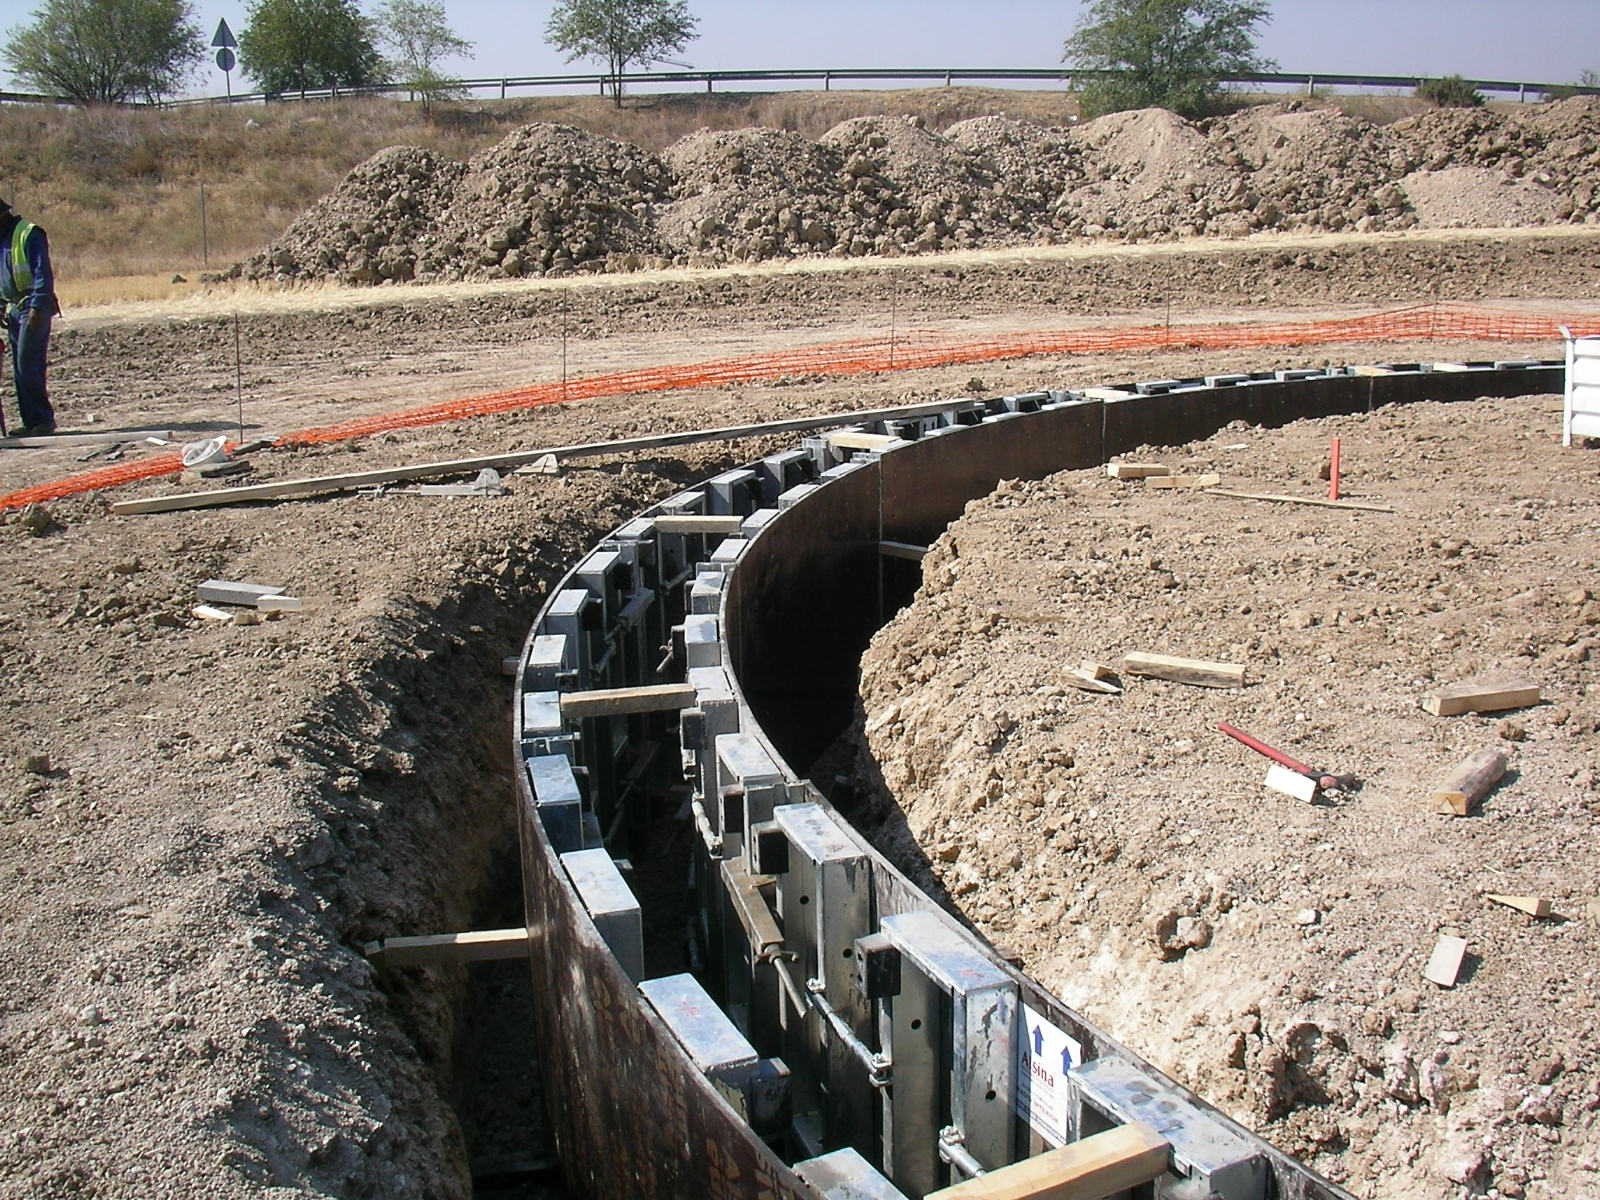
\includegraphics[width=\textwidth]{figures/1.JPG}
  \caption{Guide beam to set out the position of the sheet pile wal}
  \end{subfigure}
\hfill
  \begin{subfigure}[r]{\widhtRightCol}
  \centering
  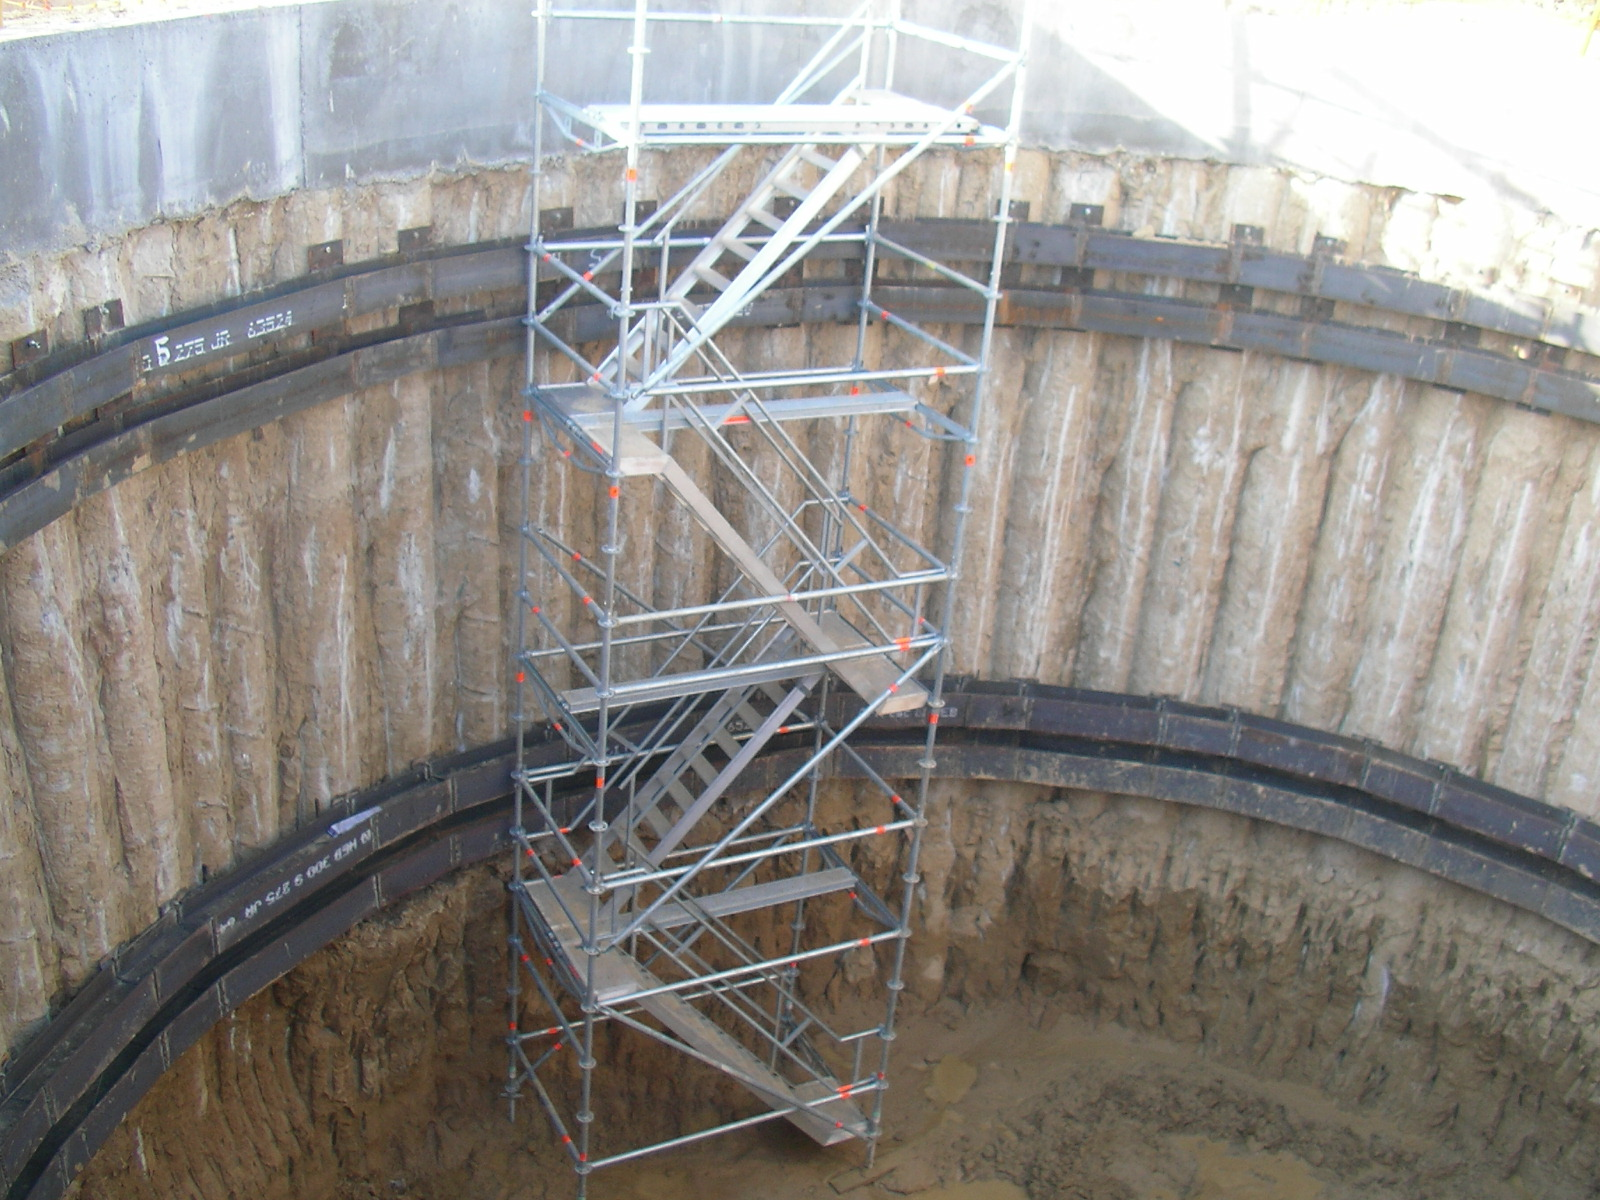
\includegraphics[width=\textwidth]{figures/2.JPG}
  \caption{Sheet of piles 55 cm in diameter, that encloses a cylindrical working shaft, 12 m diameter, 16 m depth}
  \end{subfigure}
\end{figure}

% ****

\begin{Parallel}{\widhtLeftCol}{\widhtRightCol}
  
  \ParallelLText{
 - El suelo, de acuerdo con los resultados del informe geotécnico encargado por la empresa constructora, tiene un ángulo de  rozamiento interno muy bajo (en general en torno a los $19^o$ alcanzando en algunos ensayos $13^o$).

    Con estos condicionantes, se estudió la idoneidad de las siguientes tres alternativas:

     1. Pantalla de pilotes secantes de directriz circular.
     
     2. Pantalla de paneles de hormigón armado de directriz poligonal (octogonal o similar).
     
     3. Pantalla de tablestacas de directriz circular.

 La solución de pantalla de paneles de hormigón armado quedó descartada debido a la dificultad de conseguir su estanqueidad con una directriz poligonal. Por su parte, la constructora puso objeción a la solución de tablestacas por observar dificultades para su hinca. En consecuencia se dimensionó la primera de las soluciones planteadas.

   }
  
   \ParallelRText{
     \emph{The soil, according to the results of the geotechnical report commissioned by the construction company, has a very low internal friction angle (generally around $19^o$, reaching $13^o$ in some tests).}
     
     \emph{With these restraints, the suitability of the following three alternatives was studied:}

      \emph{1. Secant pile cylindrical wall.}
     
      \emph{2. Retaining wall made of reinforced concrete panels with a polygonal guideline (octagonal or similar).}
     
      \emph{3. Sheet pile cylindrical wall.}

  \emph{The solution made of reinforced concrete panels was discarded due to the difficulty of achieving water-tightness with a polygonal guideline. On the other hand, the construction company ruled out the sheet pile solution due to difficulties regarding the driving. Consequently, the first of the proposed solutions was designed.}
     
  }
\end{Parallel}
     
\begin{figure}[h]
  \begin{subfigure}[l]{\widhtLeftCol}
  \centering
  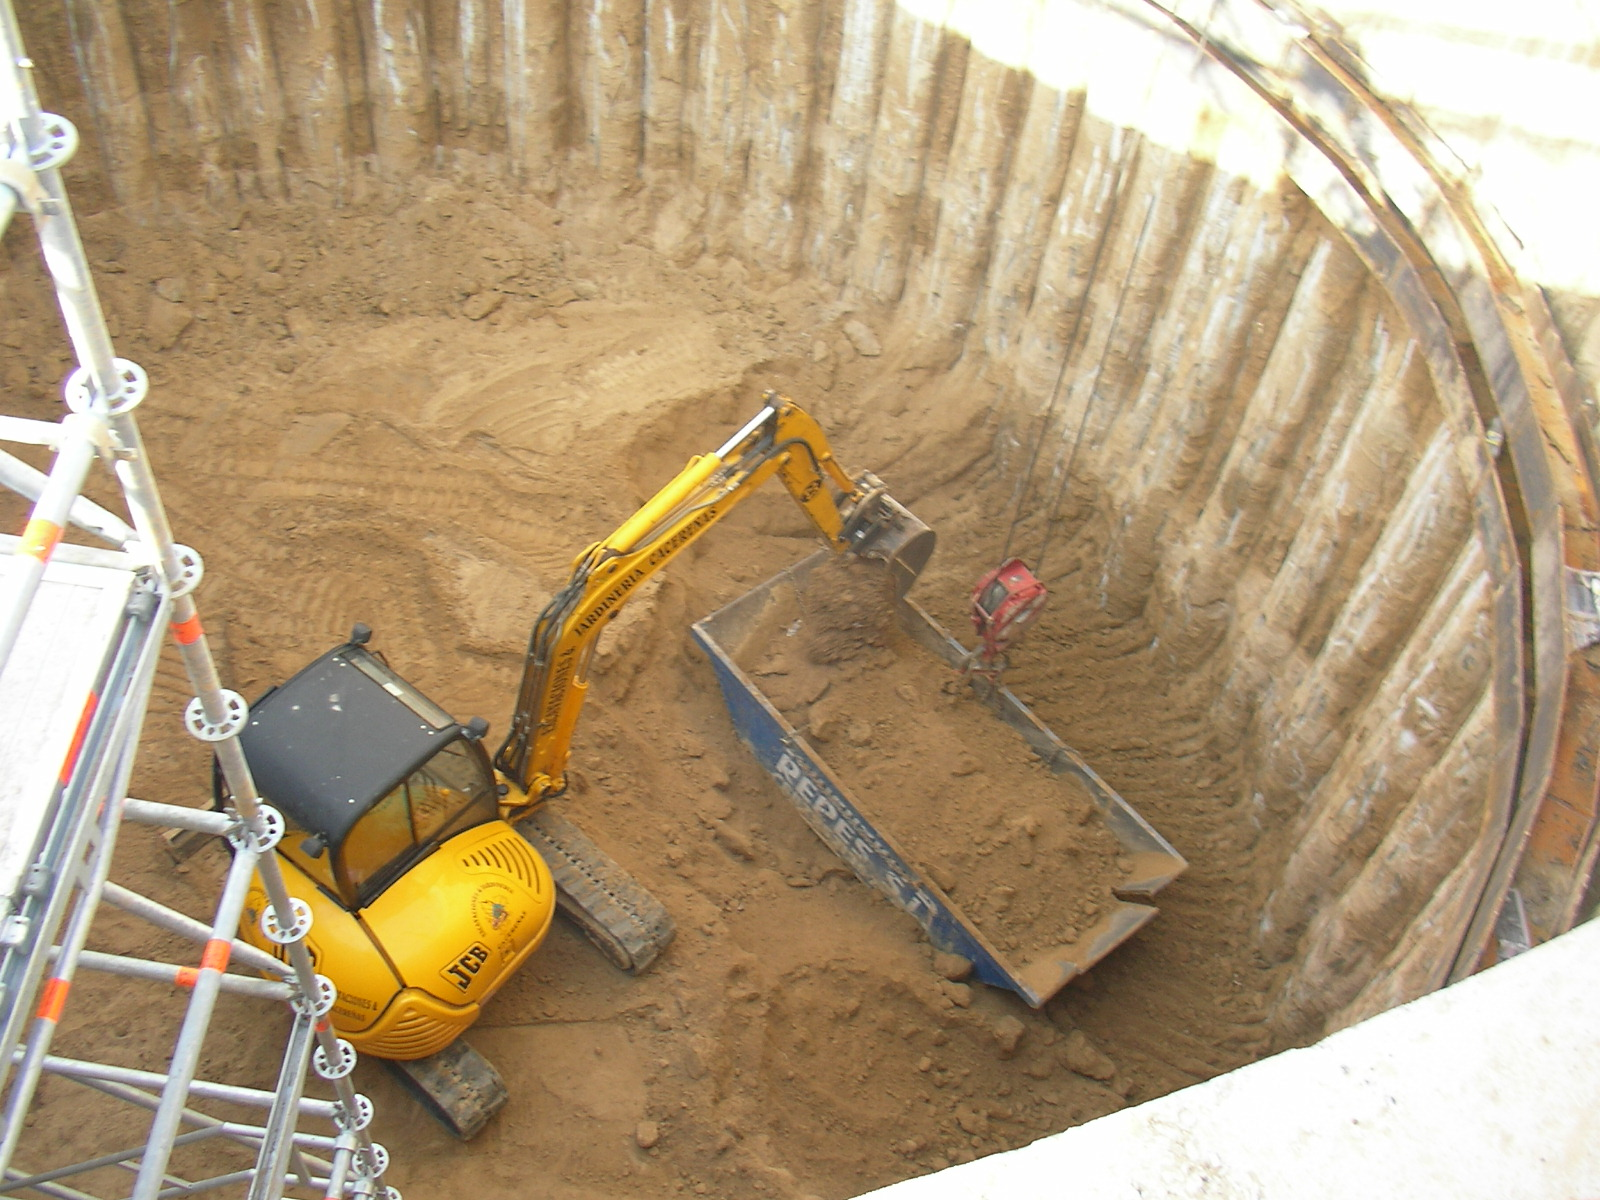
\includegraphics[width=\textwidth]{figures/3.JPG}
  \caption{Excavation of the shaft}
  \end{subfigure}
\hfill
  \begin{subfigure}[r]{\widhtRightCol}
  \centering
  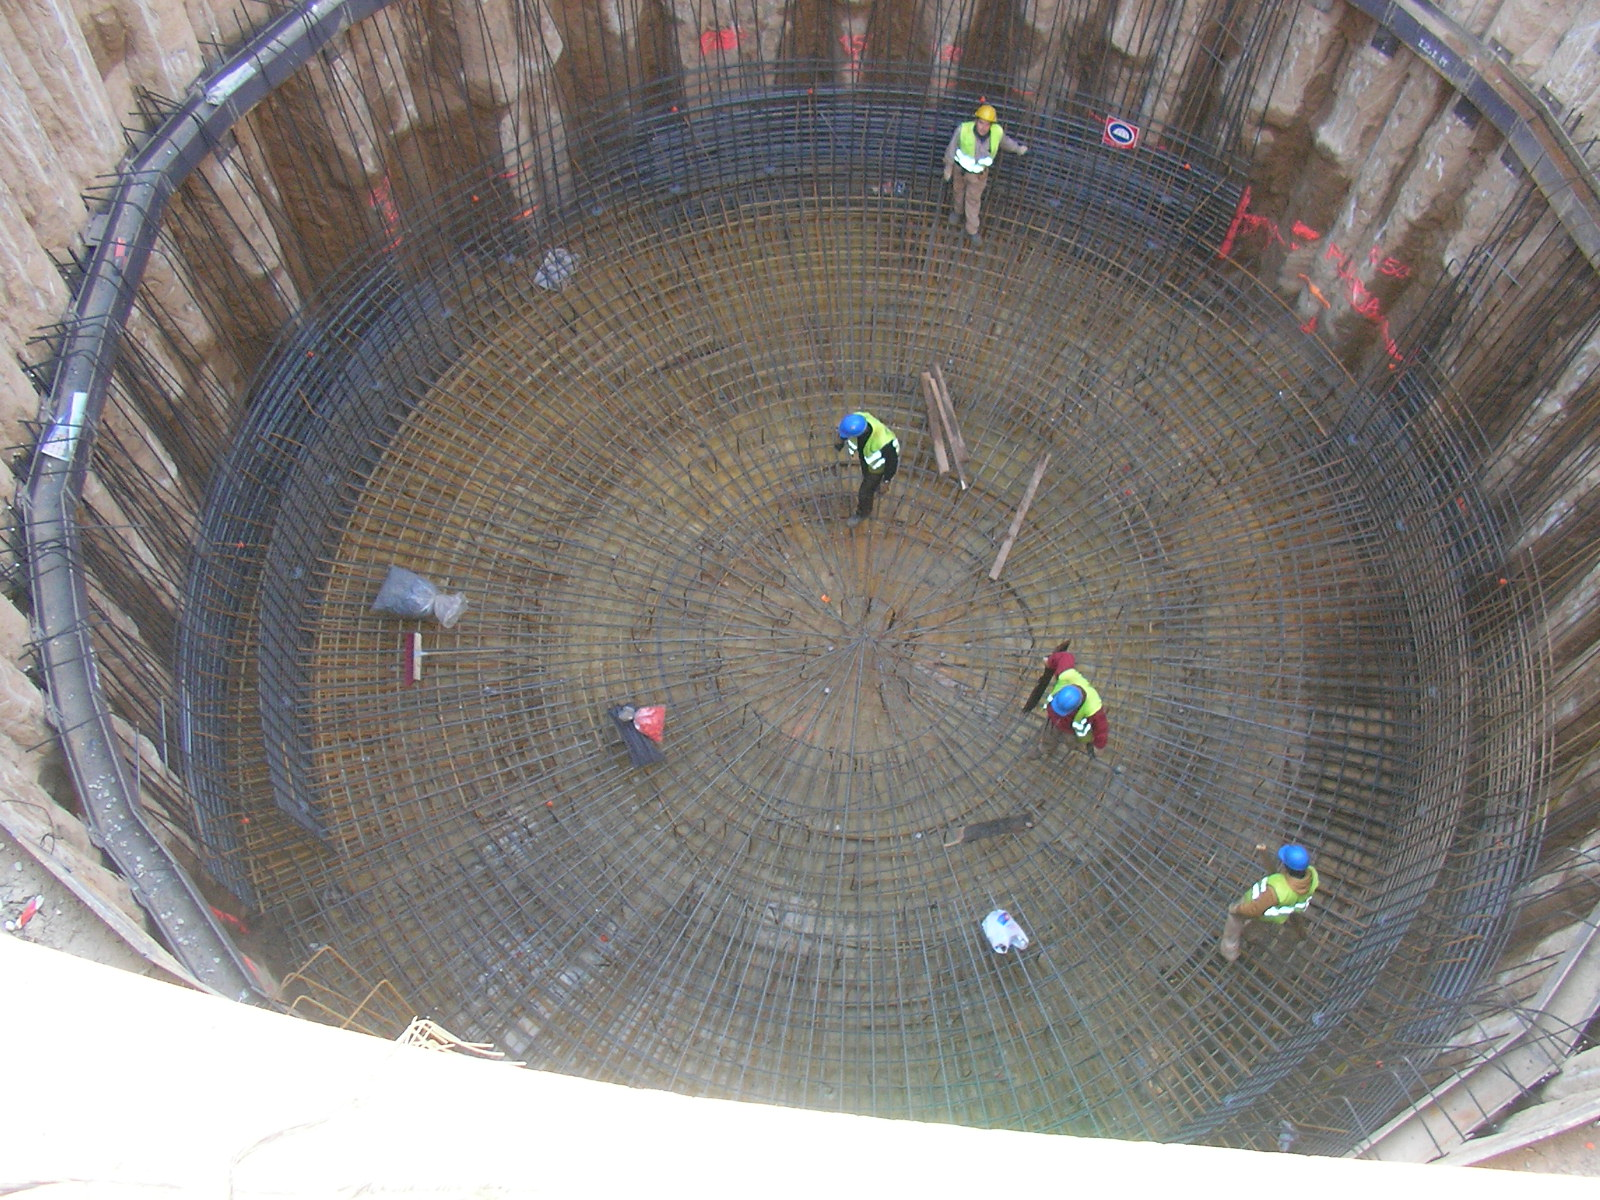
\includegraphics[width=\textwidth]{figures/4.JPG}
  \caption{Reinforcing steel placement for the construction of the foundation slab, 1.5 m in thickness.}
  \end{subfigure}
  \end{figure}

% ****

\begin{Parallel}{\widhtLeftCol}{\widhtRightCol}
   \ParallelLText{Se diseñó en primer término una pantalla de pilotes secantes de 55 cm de diámetro, la cual presentaba un excelente comportamiento frente a los empujes de tierras, resultando una armadura mínima para los pilotes secundarios. Para evitar el posible sifonamiento en el fondo de la excavación se propuso la ejecución, previamente al inicio de la excavación, de un tapón de \emph{jet grouting}. El reparto de las cargas transmitidas por los gatos entre todos los pilotes del perímetro se realizaba a través de un muro de  un macizo interior, formado por una losa inferior de 1.5 metros de espesor y un muro perimetral de 4.5 metros de altura y 1.1 metros de espesor. 

   }
  
   \ParallelRText{
     \emph{First, a 55 cm diameter secant pile wall was designed, which presented excellent behavior against earth pressure, resulting in minimal reinforcement for the secondary piles. To avoid possible siphoning at the bottom of the excavation, it was proposed to build a \emph{jet grouting} water-sealing plug before starting the excavation. The distribution of the loads transmitted by the jacks between all the piles of the perimeter was carried out through an interior solid wall, formed by a lower slab 1.5 meters thick and a perimeter wall 4.5 meters high and 1.1 meters thickness.}
  }
\end{Parallel}
     
\begin{figure}[h]
  \begin{subfigure}[l]{\widhtLeftCol}
  \centering
  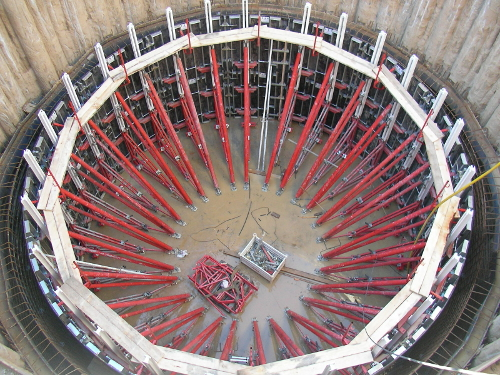
\includegraphics[width=\textwidth]{figures/5.JPG}
  \caption{Formwork for concrete wall 4.5 m high, 1.1 m thickness}
  \end{subfigure}
\hfill
  \begin{subfigure}[r]{\widhtRightCol}
  \centering
  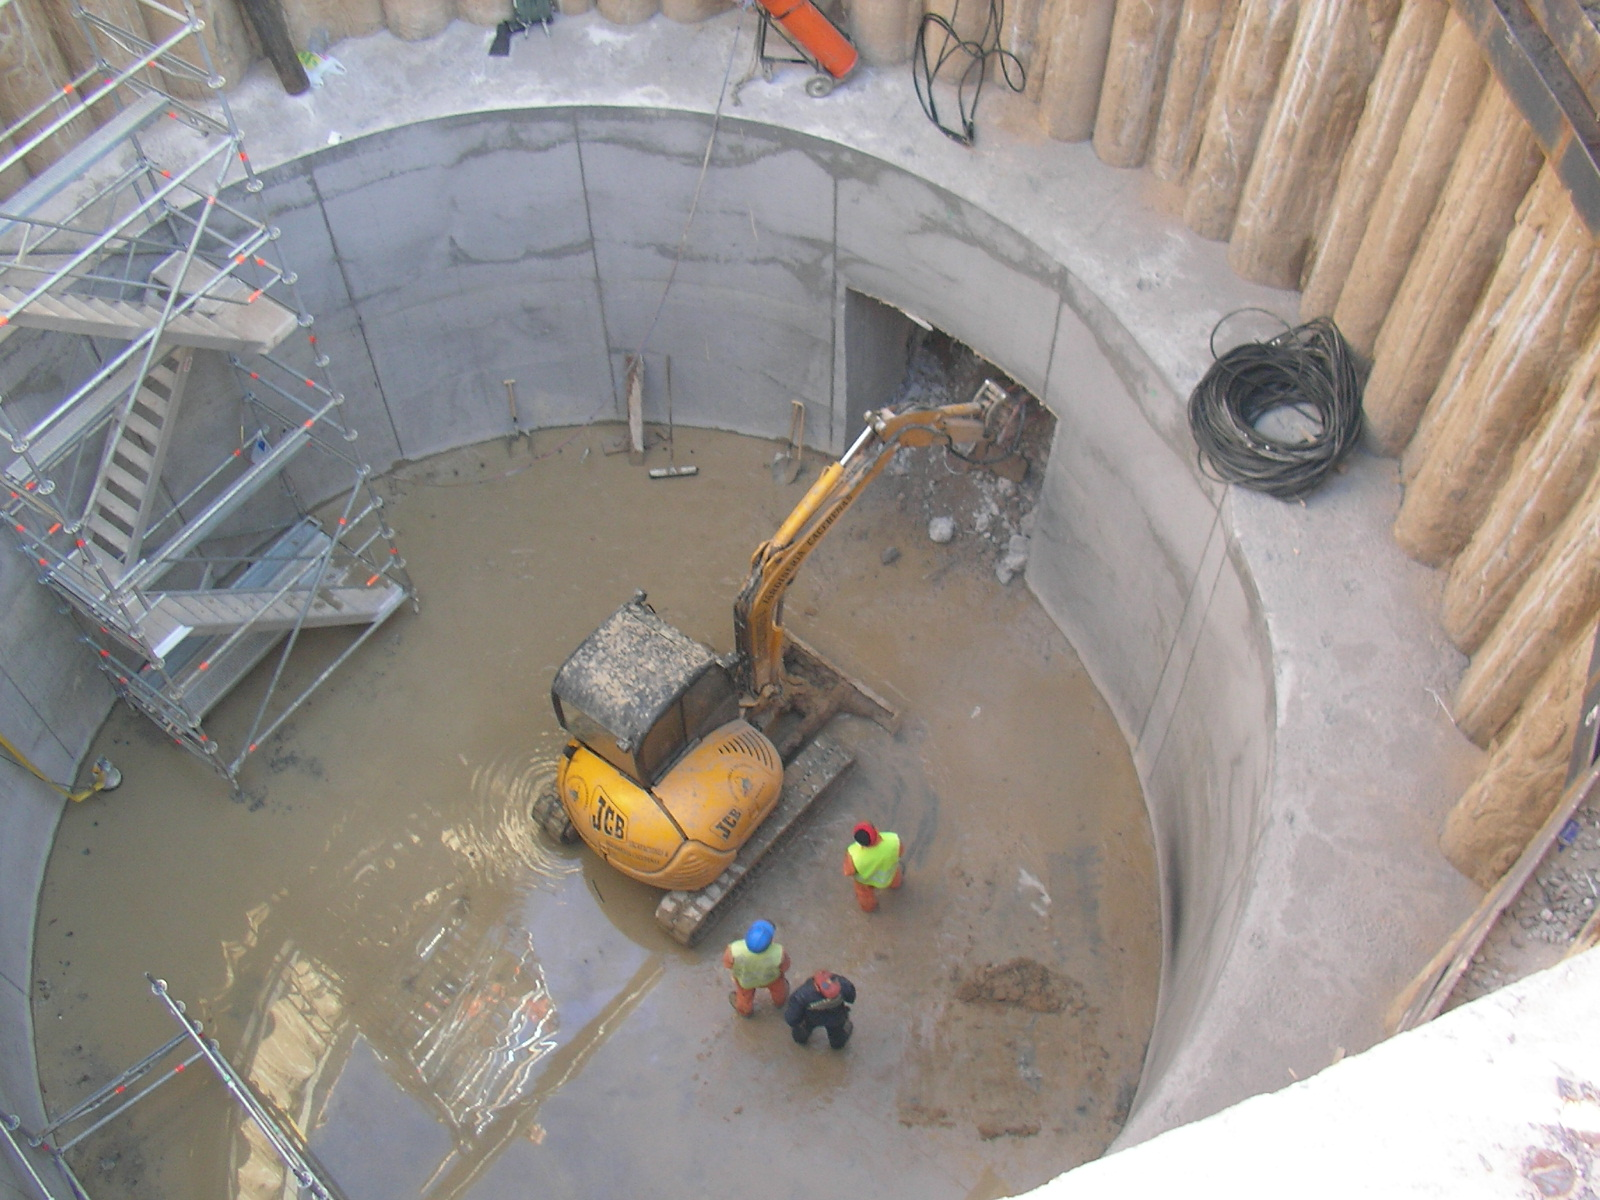
\includegraphics[width=\textwidth]{figures/6.JPG}
  \caption{Inlet of the sewer pipe}
  \end{subfigure}
  \end{figure}

% ****

\begin{Parallel}{\widhtLeftCol}{\widhtRightCol}
   \ParallelLText{Tras el inicio de la obra, se observaron una serie de dificultades para la ejecución de la solución estructural diseñada.  La coyuntura del sector de la construcción, que presentaba una gran actividad en aquel momento,  hizo que fuera imposible disponer de los medios adecuados para la ejecución de la pantalla de pilotes secantes.  En paralelo se realizó una nueva investigación geotécnica que arrojó mejores resultados del ángulo de rozamiento interno del suelo, lo que permitió construir la pantalla discontinua, formada por pilotes separados 5 cm entre sus caras, que se perforaban con barrena continua.  

   }
  
   \ParallelRText{
     \emph{Shortly after the start of the work, difficulties arose in the execution of the designed structural solution. The situation in the construction sector, which was very active at that time, made it impossible to have the right machinery for the execution of the secant pile wall. In parallel, a new geotechnical investigation was carried out that yielded better results on the internal friction angle of the soil, which allowed the construction of the discontinuous wall, formed by continuous flight auger piles, separated 5 cm between their faces.}
  }
\end{Parallel}
     
\begin{figure}[h]
  \begin{subfigure}[l]{\widhtLeftCol}
  \centering
  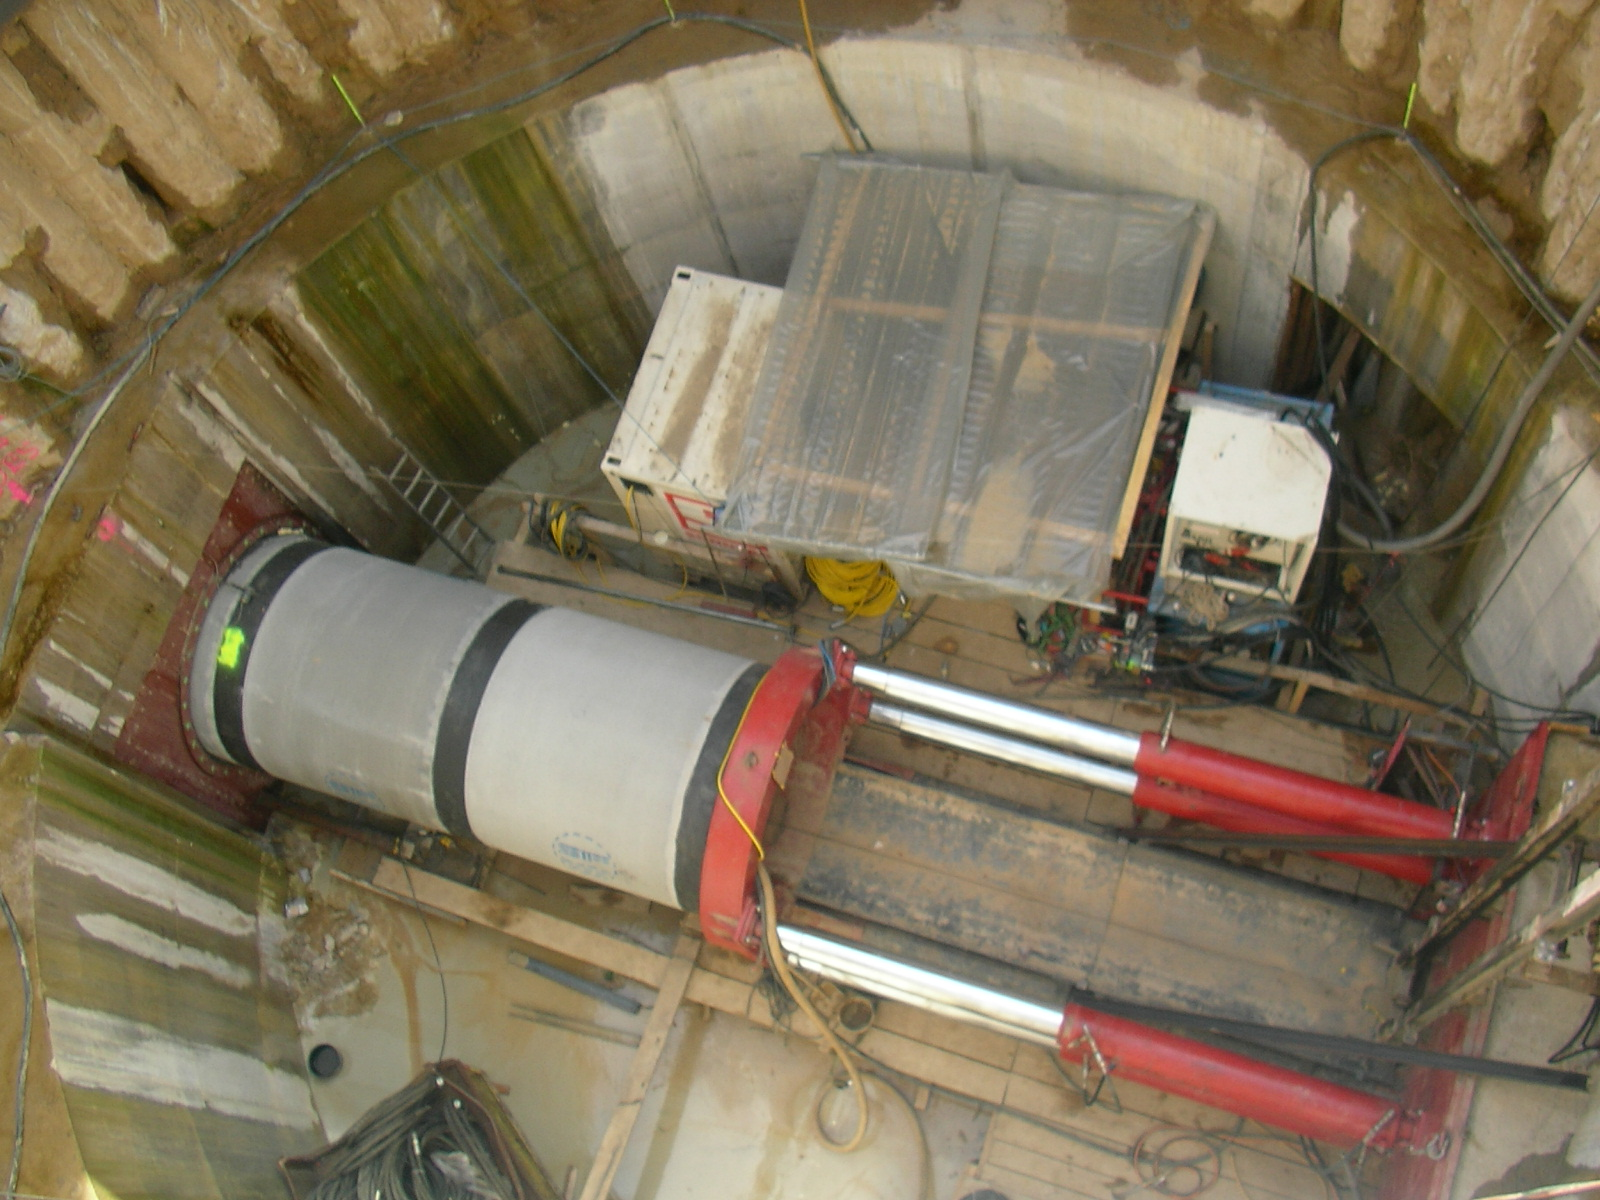
\includegraphics[width=\textwidth]{figures/7.JPG}
  \caption{Pipe jacking, withstanding a maximum thrust of 12.000 kN}
  \end{subfigure}
\hfill
  \begin{subfigure}[r]{\widhtRightCol}
  \centering
  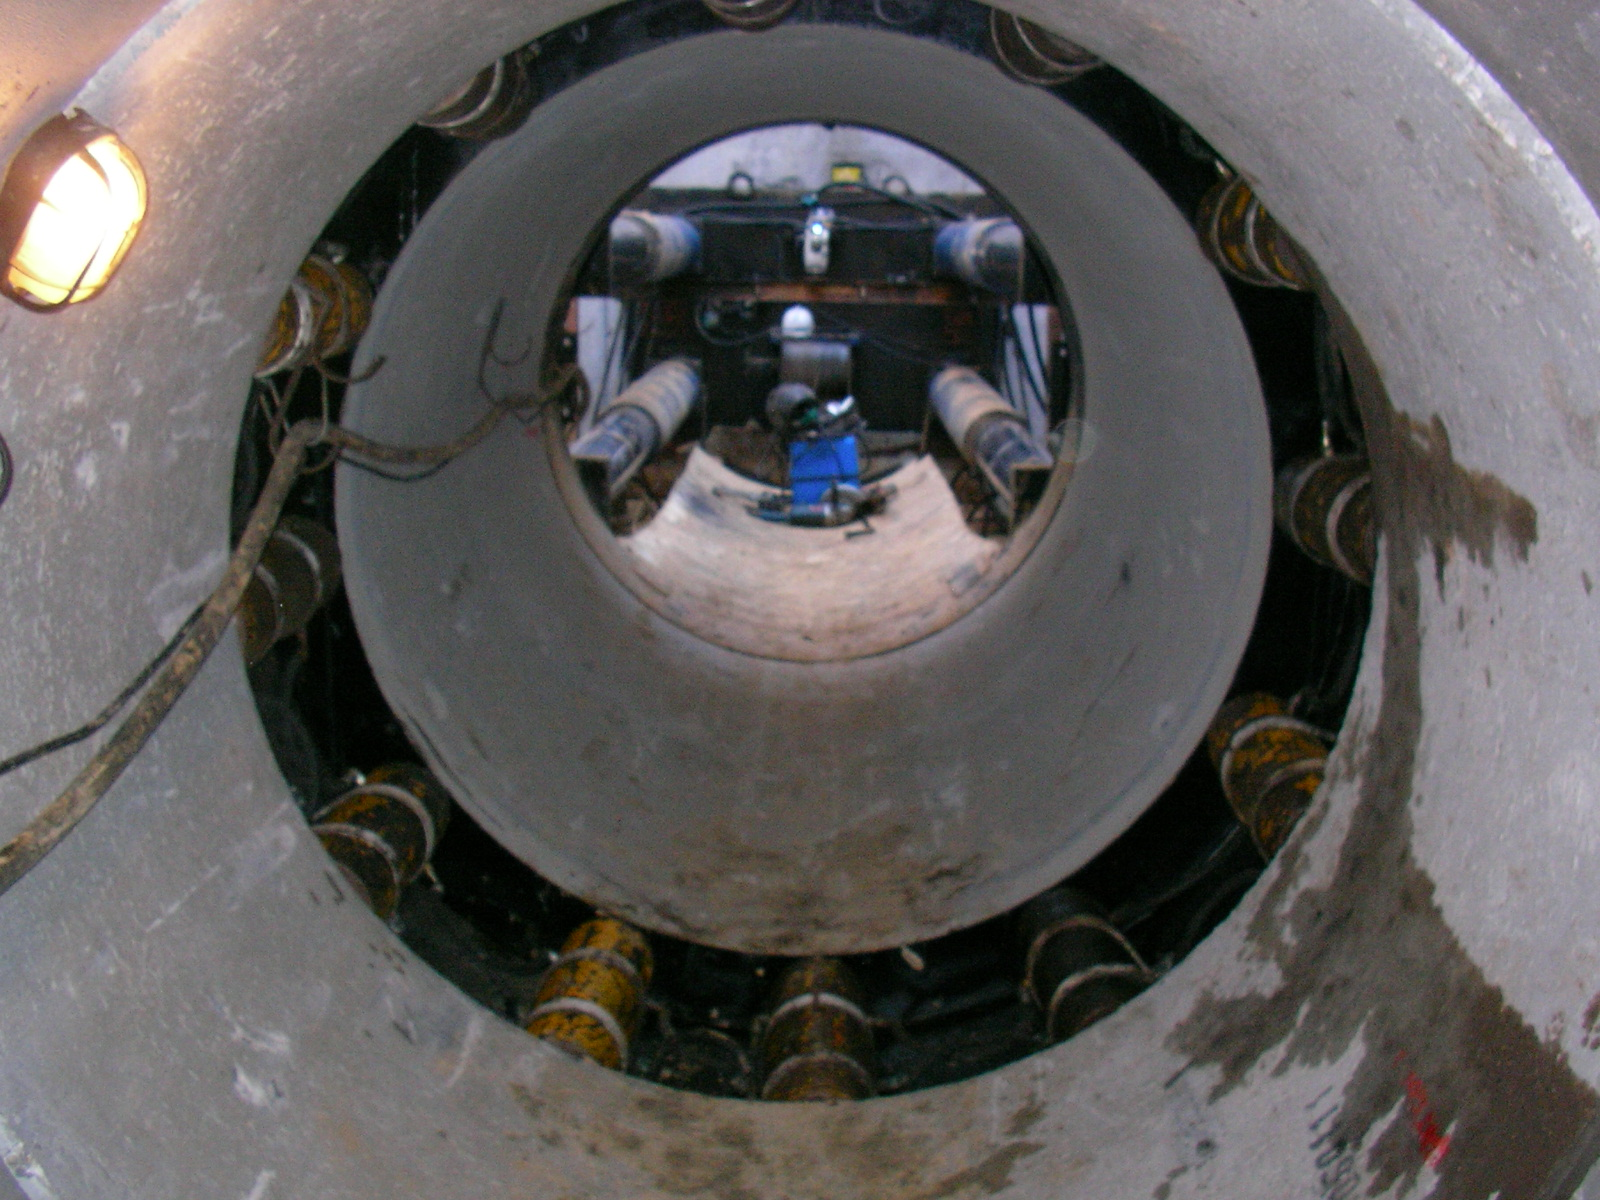
\includegraphics[width=\textwidth]{figures/8.JPG}
  \caption{Sewer pipe, 1800 mm in diameter}
  \end{subfigure}
\end{figure}

\begin{Parallel}{\widhtLeftCol}{\widhtRightCol}
  
  \ParallelLText{
    Para su ejecución, de acuerdo a los resultados del cálculo, se hizo necesario adoptar las siguientes medidas:


- Garantizar, mediante agotamiento, el rebajamiento del nivel freático por debajo  de la cota de excavación.

- Disponer varios niveles de codales a lo largo de la altura de excavación.

- Controlar desplazamientos de la pantalla durante todo el periodo de servicio de la misma.

- Evitar sobrecargas en el trasdós de la pantalla.

- Acelerar la ejecución de las últimas fases de excavación y del macizo de anclaje para que el terreno no desarrollara la totalidad del empuje.

  }
    \ParallelRText{
     \emph{For its execution, according to the results of the calculation, it was necessary to adopt the following procedures:}


\emph{- Guarantee, through pumping, the lowering of the groundwater level below the level of excavation.}

\emph{- Arrange several levels of struts along the excavation height.}

\emph{- Control the structure displacements throughout its service period.}

\emph{- Avoid overloads on the back of the shaft wall.}

\emph{- Accelerate the execution of the last phases of excavation and the inner concrete wall so that the soil does not develop the full thrust}
  }
\end{Parallel}
 
\end{document}
